\begin{exercise}
	Let $ F(x,y,z) = (y^2, xz, 1) $ be a vector field. The following curves are given:
	\begin{itemize}
		\item $ C_1: r_1(t) = (t, t, t), \quad t \in [0,1] $
		\item $ C_2: r_2(t) = (2t, 2t, 2t), \quad t \in [0, \frac{1}{2}] $
		\item $ C_3: r_3(t) = (t, t^2, t^3), \quad t \in [0,1] $
	\end{itemize}
	Sketch the curves. Compute the line integrals
	$$
		\int_{C_1} F \cdot dr, \quad \int_{C_2} F \cdot dr, \quad \int_{C_3} F \cdot dr.
	$$
	Why do the first two line integrals coincide? Is $F$ a conservative vector field?
\end{exercise}

\begin{solution}

	\begin{center}
		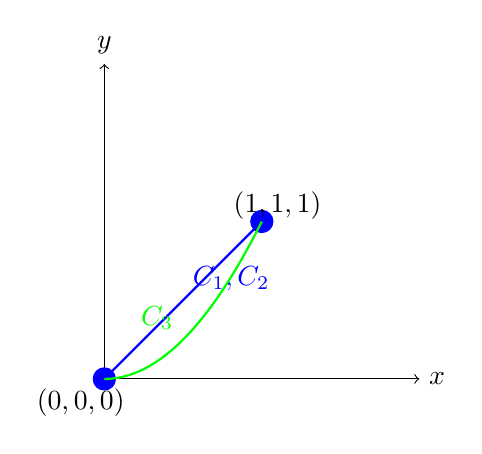
\begin{tikzpicture}[scale=2]
			\draw[->] (0,0) -- (2,0) node[right] {$x$};
			\draw[->] (0,0) -- (0,2) node[above] {$y$};

			\draw[thick, blue] (0,0) -- (1,1);
			\node[blue, above right] at (0.5, 0.5) {$C_1, C_2$};
			\filldraw[blue] (0,0) circle (2pt);
			\filldraw[blue] (1,1) circle (2pt);
			\node at (-0.15, -0.15) {$(0,0,0)$};
			\node at (1.1, 1.1) {$(1,1,1)$};

			\draw[thick, green, smooth, domain=0:1, samples=50] plot ({(\x)}, {(\x)^2});
			\node[green, above left] at (0.5, 0.25) {$C_3$};

		\end{tikzpicture}
	\end{center}

	$C_1$:
	$$
		\begin{aligned}
			r_1'(t)                 & = (1, 1, 1)                                                                               \\
			F(r_1(t))               & = (t^2, t^2, 1)                                                                           \\
			F(r_1(t)) \cdot r_1'(t) & = t^2 + t^2 + 1 = 2t^2 + 1                                                                \\
			\int_{C_1} F \cdot dr   & = \int_0^1 (2t^2 + 1) \, dt = \left[ \frac{2t^3}{3} + t \right]_0^1 = \boxed{\frac{5}{3}}
		\end{aligned}
	$$

	$C_2$:
	$$
		\begin{aligned}
			r_2'(t)                 & = (2, 2, 2)                                                                                          \\
			F(r_2(t))               & = (4t^2, 4t^2, 1)                                                                                    \\
			F(r_2(t)) \cdot r_2'(t) & = 4t^2 \cdot 2 + 4t^2 \cdot 2 + 1 \cdot 2 = 16t^2 + 2                                                \\
			\int_{C_2} F \cdot dr   & = \int_0^{1/2} (16t^2 + 2) \, dt = \left[ \frac{16t^3}{3} + 2t \right]_0^{1/2} = \boxed{\frac{5}{3}}
		\end{aligned}
	$$

	$C_3$:
	$$
		\begin{aligned}
			r_3'(t)                 & = (1, 2t, 3t^2)                                                                                                       \\
			F(r_3(t))               & = (t^4, t^4, 1)                                                                                                       \\
			F(r_3(t)) \cdot r_3'(t) & = t^4 + 2t^5 + 3t^2                                                                                                   \\
			\int_{C_3} F \cdot dr   & = \int_0^1 (t^4 + 2t^5 + 3t^2) \, dt = \left[ \frac{t^5}{5} + \frac{t^6}{3} + t^3 \right]_0^1 = \boxed{\frac{23}{15}}
		\end{aligned}
	$$

	\bigskip
	$C_1$ and $C_2$ represent the same geometric curve despite different parametrizations. The line integral is independent of parametrization; it depends only on the geometric path and endpoints.

	\bigskip
	\noindent To show: $F$ is not conservative

	\noindent Proof:
	$$
		F \text{ conservative} \iff \nabla \times F = 0
	$$
	$$
		\begin{aligned}
			\nabla \times F & = \begin{pmatrix} \frac{\partial}{\partial x} \\ \frac{\partial}{\partial y} \\ \frac{\partial}{\partial z} \end{pmatrix} \times \begin{pmatrix} y^2 \\ xz \\ 1 \end{pmatrix}                                                               \\
			                & = \begin{pmatrix} \frac{\partial(1)}{\partial y} - \frac{\partial(xz)}{\partial z} \\ \frac{\partial(y^2)}{\partial z} - \frac{\partial(1)}{\partial x} \\ \frac{\partial(xz)}{\partial x} - \frac{\partial(y^2)}{\partial y} \end{pmatrix} \\
			                & = \begin{pmatrix} 0 - x \\ 0 - 0 \\ z - 2y \end{pmatrix} \neq 0
		\end{aligned}
	$$

\end{solution}
